\documentclass{article}
\usepackage{amsmath}
\usepackage[utf8]{inputenc}
\usepackage[T1]{fontenc}
\usepackage[ngerman]{babel}
\usepackage[shortlabels]{enumitem}
\usepackage{amsfonts}
\usepackage[left=3cm,right=2cm,top=2.5cm,bottom=2cm]{geometry}
\usepackage{amssymb}
\usepackage{cancel}
\usepackage{karnaugh-map}
\usepackage{xcolor}
\usepackage{caption}
\usepackage{subcaption}
\usepackage{tikz}

\newcommand{\nyet}{\overline}

\title{Formale Grundlagen: Übung 5}
\author{Alexander Waldenmaier, Tutorin: Constanze Merkt}

\begin{document}
    \maketitle

    \subsection*{Aufgabe 5.1}
    \begin{table*}[h]
        \centering
        \begin{tabular}{ccc|c}
            $x$ & $y$ & $z$ & f \\ \hline
            0 & 0 & 0 & 0 \\
            0 & 0 & 1 & 1 \\
            0 & 1 & 0 & 1 \\
            0 & 1 & 1 & 0 \\
            1 & 0 & 0 & 1 \\
            1 & 0 & 1 & 0 \\
            1 & 1 & 0 & 0 \\
            1 & 1 & 1 & 1
        \end{tabular}
    \end{table*}


    \subsection*{Aufgabe 5.2}
    \begin{minipage}[h]{0.6\textwidth}
        Die ersten $n$ Eingänge des Perzeptrons werden an die $n$ Bits der Zahl $x$ angeschlossen, genauso werden die darauffolgenden $n$ Bits mit der Zahl $y$ verknüpft. Als Gewichte dienen für die $x$-Bits in aufsteigender Reihenfolge für $\{x_0, x_1, \ldots, x_{n-1}\}$ die Werte $\{2^0, 2^1, \ldots , 2^{n-1}\}$. Die $y$-Bits erhalten die selben Gewichte in der selben Reihenfolge, allerdings mit negativem Vorzeichen. Wählt man nun einen Schwellwert $t=0$, bildet man die Funktion $x \ge y$ ab. Für den Fall $f(x, y)= x>y$ muss ein Wert im Intervall $(0,1)$ gewählt werden, beispielsweise $t=0,5$.
    \end{minipage}
    \begin{minipage}[h]{0.35\textwidth}
        \hspace{0.5cm}
        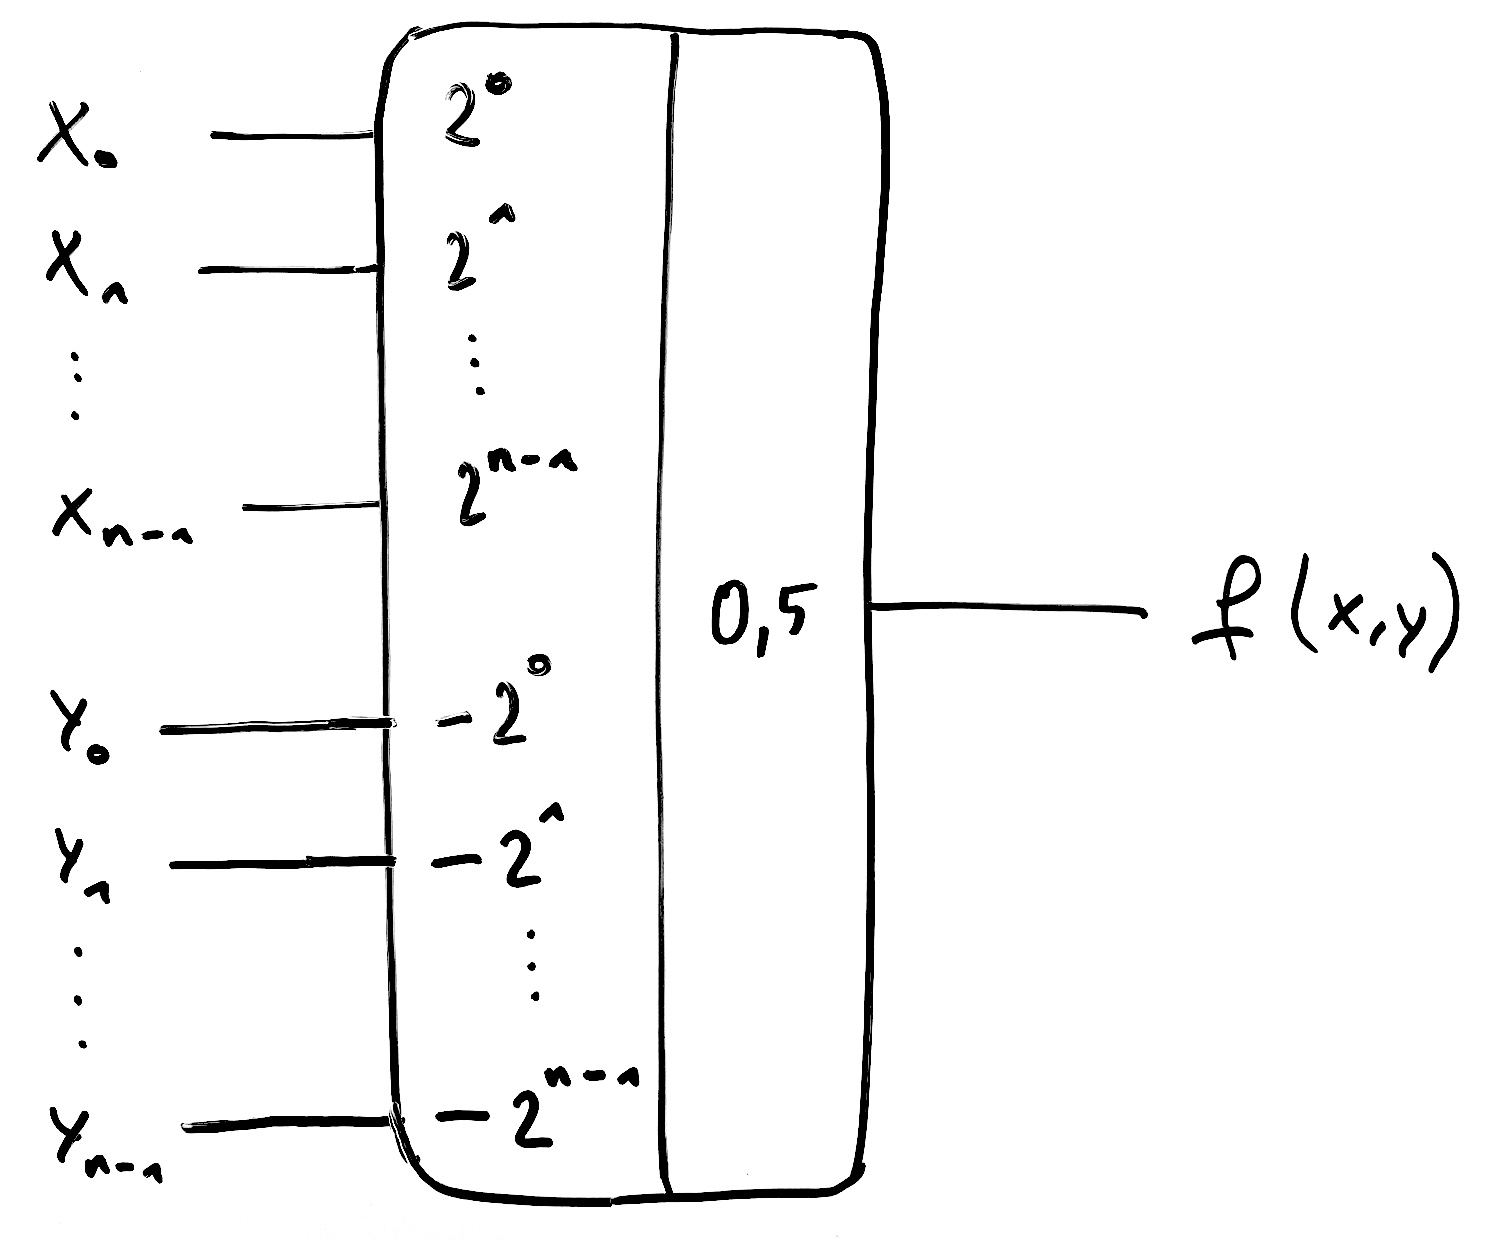
\includegraphics[width=0.9\textwidth]{perzeptron.jpeg}
    \end{minipage}



    \subsection*{Aufgabe 5.3}
    Die Aussage stimmt nicht. Die Funktionen $f(x_1, x_2) = \overline{x_1} + x_2$ und $g(x_1, x_2) = x_1 + \nyet{x_2}$ sind jeweils linear separierbar, wie in den Abbildungen a) und b) veranschaulicht. Deren Konjunktion, $f \land g$, ist es hingegen nicht (XNOR-Funktion, siehe Abbildung c)). 
    \begin{figure}[h]
        \centering
        \begin{subfigure}[b]{0.3\textwidth}
            \centering
            \begin{tikzpicture}
                \draw 
                    (0,0) node[below left]{(0,0)} -- 
                    (2,0) node[below right]{(1,0)} -- 
                    (2,2) node[above right]{(1,1)} -- 
                    (0,2) node[above left]{(0,1)} -- 
                    cycle;
                \draw[dashed] (-0.5,1) -- (1, 2.5);
                \draw[fill=black] (0,0) circle (3pt);
                \draw[fill=black] (2,0) circle (3pt);
                \draw[fill=black] (2,2) circle (3pt);
                \draw[fill=white] (0,2) circle (3pt);
            \end{tikzpicture}
            \caption{$f(x_1, x_2)$}
        \end{subfigure}
        \begin{subfigure}[b]{0.3\textwidth}
            \centering
            \begin{tikzpicture}
                \draw 
                    (0,0) node[below left]{(0,0)} -- 
                    (2,0) node[below right]{(1,0)} -- 
                    (2,2) node[above right]{(1,1)} -- 
                    (0,2) node[above left]{(0,1)} -- 
                    cycle;
                \draw[dashed] (1,-0.5) -- (2.5, 1);
                \draw[fill=black] (0,0) circle (3pt);
                \draw[fill=white] (2,0) circle (3pt);
                \draw[fill=black] (2,2) circle (3pt);
                \draw[fill=black] (0,2) circle (3pt);
            \end{tikzpicture}
            \caption{$g(x_1, x_2)$}
        \end{subfigure}
        \begin{subfigure}[b]{0.3\textwidth}
            \centering
            \begin{tikzpicture}
                \draw 
                    (0,0) node[below left]{(0,0)} -- 
                    (2,0) node[below right]{(1,0)} -- 
                    (2,2) node[above right]{(1,1)} -- 
                    (0,2) node[above left]{(0,1)} -- 
                    cycle;
                \draw[fill=black] (0,0) circle (3pt);
                \draw[fill=white] (2,0) circle (3pt);
                \draw[fill=black] (2,2) circle (3pt);
                \draw[fill=white] (0,2) circle (3pt);
            \end{tikzpicture}
            \caption{$f(x_1, x_2) \land g(x_1, x_2)$}
        \end{subfigure}
    \end{figure}
    

    \subsection*{Aufgabe 5.4}
    Das Verfahren könnte bereits bei $i=5$ abgebrochen werden. Der Vollständigkeit halber sind allerdings die Zeilen $i=6$ und $i=7$ ebenfalls dargestellt (mit unveränderten Gewichten), die aufzeigen, dass alle Vektoren $a, b, c$ nun korrekt kategorisiert werden. 
    \begin{table*}[h]
        \centering
        \begin{tabular}{c|ccccc|ccccc|ccc|c}
            $i$ & $w_0^{(i)}$ & $w_1^{(i)}$ & $w_2^{(i)}$ & $w_3^{(i)}$ & $w_4^{(i)}$ & $y_0$ & $y_1$ & $y_2$ & $y_3$ & $y_4$ & $\mathbf{yw}^{(i)}$ & $>0$ & $\mathbf{y} \in Y_1$ \\ \hline \hline
            0 &   0 & 0 & 0 & 0 & 0 &   1 & 1 & 1 & 1 & 0   & 0 & 0 & 1 \\
            1 &   1 & 1 & 1 & 1 & 0 &   1 & 0 & 0 & 1 & 1   & 2 & 1 & 0 \\
            2 &   0 & 1 & 1 & 0 & 0 &   1 & 1 & 0 & 1 & 0   & 1 & 1 & 0 \\ 
            \hline
            3 &  -1 & 0 & 1 &-1 & 0 &   1 & 1 & 1 & 1 & 0   &-1 & 0 & 1 \\
            4 &   0 & 1 & 2 & 0 & 0 &   1 & 0 & 0 & 1 & 1   & 0 & 1 & 0 \\
            5 &  -1 & 1 & 2 &-1 &-1 &   1 & 1 & 0 & 1 & 0   &-1 & 0 & 0 & \checkmark \\
            \hline
            6 &  -1 & 1 & 2 &-1 &-1 &   1 & 1 & 1 & 1 & 0   & 1 & 1 & 1 & \checkmark \\
            7 &  -1 & 1 & 2 &-1 &-1 &   1 & 0 & 0 & 1 & 1   &-3 & 0 & 0 & \checkmark\\
        \end{tabular}
    \end{table*}
    

    \subsection*{Aufgabe 5.5}
    Generell gilt: Boolsche Funktionen lassen sich genau dann mit nur einem Perzeptron darstellen, wenn sie linear separierbar sind. 
    \begin{enumerate}
        \item[a)] Der eindimensionale Werteraum hat die Werte $\{1, 0\}$ die mit den Werten $\{0, 1\}$ aus dem Definitionsbereich in entsprechender Reihenfolge bijektiv verknüpft sind. Folglich lässt sich die der Wertebereich durch einen beliebigen Punkt im Intervall $(0,1)$ separieren. 
        \item[b)] Man stelle sich sich den Argumentenraum $\{x_1, \ldots, x_n\}$ in der Form eines Hyperwürfels vor (Quadrat für $n=2$, Würfel für $n=3$), dessen Eckpunkte sämtliche Wertekombinationen von $\mathbf{x}$ darstellen. Bei $f$ gibt es nun genau einen solchen Eckpunkt, und zwar den für $\mathbf{x} = 1$, bei dem die Funktion 1 ergibt, sonst ist die Konjunktion stets 0. Bei der Funktion $g$ ist es umgekehrt: Es existiert genau ein Eckpunkt, und zwar der für $\mathbf{x} = 0$, für den die Disjunktion 0 ergibt, sonst ist sie stets 1. 
        
        Ein einzelner Eckpunkt lässt sich immer durch eine geeignete Hyperebene von allen anderen Punkten abtrennen, da seine konvexe Hülle disjunkt von der konvexen Hülle der Menge aller anderen Punkte ist. Folglich sind die Funktionen $f$ und $g$ linear separierbar. 
        \item[c)] Jede Funktion $f$ lässt sich beispielsweise in der DNF darstellen, in der nur Komplemente, Konjunktionen und Disjunktionen enthalten sind. 
        
        In der ersten Ebene eines generellen DNF-kompatiblen Perzeptronen-Schaltkreises befinden sich $\le n$ Inverter, die alle Eingänge, die auch in inverser Form gebraucht werden, umgekehren. Dies ist jeweils durch nur ein Perzeptron realisierbar, wie in a) gezeigt wurde.

        Nun können die Minterme reproduziert werden, indem für jeden Term ein eigenes UND-Perzeptron verwendet wird. Diesem werden alle erfordelichen Literale (ggf. aus dem Inverter kommend) übergeben. Anschließend werden alle diese "`Minterm-Perzeptrone"' in der dritten Ebene einem finalen ODER-Perzeptron übergeben, welches alle Minterme in Disjunktion stellt und als Ausgang den gewünschten Funktionswert von $f$ liefert. Die UND- bzw. ODER-Schaltungen sind mit je nur einem Perzeptron realisierbar, wie in b) gezeigt wurde.

        Da Inverter in Ebene 1, die UND-Perzeptrone in Ebene 2 und das ODER-Perzeptron in Ebene 3 alle jeweils innerhalb ihrer Ebene parallel ablaufen, ist die Tiefe eines solchen Schaltkreises nur 3. Hätte man es mit einer Funktion zu tun, die keinerlei invertierte Literale beinhaltet, so könnte man sogar die erste Ebene weglassen und erhielte eine Tiefe von 2. Gäbe es nur einen Minterm, könnte auch die letzte Ebene weggelassen werden wodurch die Tiefe sogar 1 wäre. 
    \end{enumerate}
\end{document}